\section{Data}\label{sec:data}

\subsection{Ethereum Event Logs and Meta-Events}\label{sec:data-event-logs}

The Ethereum event logs record specific occurrences or outputs
generated during the execution of contract code.  They enable
off-chain applications to react to on-chain events.  A popular event
is the \texttt{Transfer} event emitted by ERC~20
tokens~\cite{vogelsteller-buterin-15}:

\begin{lstlisting}[language=Solidity,
    caption={The ERC~20 \texttt{Transfer} event specifies three
      parameters: \texttt{from}, \texttt{to}, and \texttt{value}.}]
  event Transfer(address indexed from,
                 address indexed to,
                 uint256 value);
\end{lstlisting}

The event has two special cases.  In the first, the \texttt{from}
address is the zero address (\texttt{0x0}) and the contract mints new
tokens.  In the second, the \texttt{to} address is the zero address
and the contract burns existing tokens.

A single transaction can emit multiple events.  We define a
\textit{meta-event} to be a sequence of events that match some pattern
and are emitted by a single transaction.  We define a
\textit{tokenising meta-event} to be a meta-event where the pattern is
two \texttt{Transfer} events: one must indicate a transfer of tokens
to the contract and another must indicate a new token being minted
(\textit{deposit \& mint}), or one must indicate a token being burned
and another must indicate a transfer of an existing token from the
contract (\textit{withdraw \& burn}.  Our aim is to identify instances
where a token is tokenised by another token.  In the terminology of
ERC~4626, a tokenising meta-event corresponds to either a
\texttt{Deposit} event or a \texttt{Withdraw} event.  However, our
tokenising meta-event does not require the contract to follow
ERC~4626.

\begin{table*}
  \centering
  \caption{Each tokenising meta-event contains the address of the
    source token, the address of the target token, one of two possible
    pairs of actions (deposit \& mint or withdraw \& burn), the amount
    of the source token that was deposited or withdrawn, the amount of
    the target token that was minted or burned, and a transaction
    hash.  The table includes four sample entries from the full set of
    \num{4032033} tokenising meta-events: the earliest and latest
    tokenising meta-events that have deposit \& mint and withdraw \&
    burn actions.}\label{tab:meta-events}
  \begin{tabular}{|c|c|c|r|r|c|}
    \hline
    Source Token &
    Target Token &
    Actions &
    Source Amount &
    Target Amount &
    Tx Hash\\
    \hline

    % 0x549a1226da1eadc6f1af7c41aef6adc638466ffd8630822637706632bf8666d3:
    % First deposit/mint.
    \texttt{ARC}~(\texttt{0xac709f}) &
    \texttt{SWT}~(\texttt{0xb12a3c}) & deposit \& mint & \textit{dust}
    & \textit{dust} & \texttt{0x549a12}\\

    % 0x2da2326c330cb1fa1330151b60453448e19b02981e45fb5dc2ed0980224ce625:
    % First withdraw/burn.
    \texttt{DGZ}~(\texttt{0x84178d}) &
    \texttt{preDGZ}~(\texttt{0x18aa6e}) & withdraw \& burn &
    \num{1371} & \num{150} & \texttt{0x2da232}\\

    % 0x5dbe32de3b682fc1c7dc181fbf74eabbb87583c4bdce371c2a997c54fca47bfb:
    % Last withdraw/burn.
    \texttt{BONE}~(\texttt{0x981303}) &
    \texttt{tBONE}~(\texttt{0xf7a038}) & withdraw \& burn & \num{5183}
    & \num{5160} & \texttt{0x5dbe32}\\

    % 0xb4281adc73ca60aef5c29e0ae7114d629c3769b7cf9fcf9e365f6cb140c8527a:
    % Last deposit/mint.
    \texttt{WETH}~(\texttt{0xc02aaa}) &
    \texttt{aWETH}~(\texttt{0x030ba8}) & deposit \& mint & \num{25} &
    \num{25} & \texttt{0xb4281a}\\

    \hline
  \end{tabular}
\end{table*}

We extracted all \texttt{Transfer} events from Ethereum mainnet from
block height \num{0} to \num{16685101} (February 2023) inclusive using
Geth's \texttt{eth\_getLogs} RPC method~\cite{geth-xx}.  From the
\texttt{Transfer} events, we identified \num{4032033} tokenising
meta-events using the pattern described above.
Table~\ref{tab:meta-events} shows a sample of the data.  The first
(resp., last) two rows are the earliest (resp., latest) two
occurrences of tokenising meta-events in the data that perform a
deposit \& mint, and a withdraw \& burn.

For example, the first row indicates a transaction that deposited a
dust amount of ARC~\cite{arcade-city-xx} to a contract in a one-to-one
exchange for newly minted SWT~\cite{swarm-city-xx} in January 2017.
The third row indicates a transaction that withdrew
\num{5183}~{BONE}~\cite{shiba-inu-xx} from a contract in exchange for
burning \num{5160}~\texttt{tBONE} in February 2023.  We are not
concerned with the individual utility or value of the tokens (or lack
thereof); we are only interested in the fact that Token~$\mathcal{X}$
can be deposited with a contract to mint Token~$\mathcal{Y}$, and/or
Token~$\mathcal{Y}$ can be burned by a contract to withdraw
Token~$\mathcal{X}$.

We filter the tokenising meta-events to include only those meta-events
that involve two tokens, Token~$\mathcal{X}$ and Token~$\mathcal{Y}$,
such that there is at least one instance of Token~$\mathcal{X}$ being
deposited with a contract to mint Token~$\mathcal{Y}$, and at least
one instance of Token~$\mathcal{Y}$ being burned by a contract to
withdraw Token~$\mathcal{X}$.  In other words, the ``and/or''
conjunction in the previous paragraph is replaced by ``and''.  This
excludes \textit{one-way token upgrades} where Token~$\mathcal{X}$ can
be deposited with a contract to mint Token~$\mathcal{Y}$ but
Token~$\mathcal{X}$ cannot be withdrawn from the contract, and
\textit{one-way token burns} where Token~$\mathcal{Y}$ can be burned
by a contract to withdraw Token~$\mathcal{X}$ but Token~$\mathcal{X}$
cannot be deposited with the contract to mint Token~$\mathcal{Y}$.  Of
the \num{4032033} tokenising meta-events, \num{3461723} meet the
additional criterion.  We will refer to the unfiltered and filtered
tokenising meta-events in Sect.~\ref{sec:data-token-graphs}.

\subsection{Off-Chain Data}\label{sec:data-off-chain}

CoinGecko~\cite{gecko-labs-xx} is a cryptocurrency data platform that
aggregates fundamental analysis of tokens including market price,
exchange volume, and market capitalisation.

DEX Screener~\cite{dex-screener-xx} stores, parses, and analyses
blockchain data to produce a token screener, charts, and analytics.
They cover many blockchains, decentralised exchanges, and tokens.

\subsection{The Token Graphs}\label{sec:data-token-graphs}

\begin{figure}
  \centerline{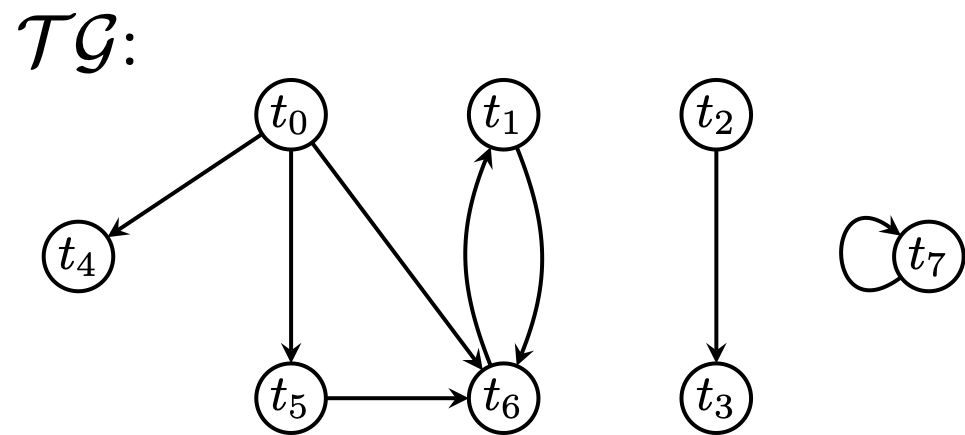
\includegraphics[width=0.8\columnwidth]{img/token-graph/token-graph.png}}
  \caption{A token graph, $\mathcal{TG}$, with eight vertices, $t_0,
    t_1, \ldots, t_7$, and eight edges.  Each edge corresponds to a
    token tokenising another token.  For example, the token
    represented by $t_5$ tokenises the token represented by $t_0$.
    The graph contains an undirected cycle ($t_0, t_5, t_6$), a
    directed cycle ($t_1, t_6$), and a loop ($t_6$).
  }\label{fig:token-graph}
\end{figure}

We can construct a directed graph from the tokenising meta-events as
follows.  Each vertex corresponds to a distinct token.  Each directed
edge from a source vertex to a target vertex corresponds to a set of
tokenising meta-events that deposits the source token and mints the
target token, and/or withdraws the source token and burns the target
token.  In the terminology of ERC~4626, the source token is the
\textit{asset} and the target token is the \textit{share}.
Figure~\ref{fig:token-graph} shows an example token graph.

In the unfiltered case, the directed graph has \num{23687} vertices
(distinct tokens) and \num{23549} edges representing pairs of tokens
where the second tokenises the first with either deposit \& mint or
withdraw \& burn actions.  In the filtered case, the directed graph
has \num{8424} vertices that are incident with at least one edge and
\num{7536} edges representing pairs of tokens where the second
tokenises the first with both deposit \& mint and withdraw \& burn
actions.  We will refer to the unfiltered and filtered token graphs in
the remainder of the paper.

\subsection{Data Limitations}\label{sec:data-limitations}

Our input data, namely, Ethereum event logs, CoinGecko market data,
and DEX Screener liquidity pool data, have limitations.  Firstly,
Ethereum event logs are unauthenticated: a contract can emit an event
of its choosing.  There is no guarantee that, say, an ERC-20
\texttt{Transfer} event accurately reflects an actual
transfer~\cite{guidi-michienzi-22}.  Additionally, the first special
case highlighted in Sect.~\ref{sec:data-event-logs} is stipulated by
ERC-20\footnote{``A token contract which creates new tokens SHOULD
trigger a Transfer event with the \texttt{\_from} address set to
\texttt{0x0} when tokens are
created.''~\cite{vogelsteller-buterin-15}} but the second is not.
However, event logs are generally accurate and malicious contracts can
be easily excluded.  For an aggregated analysis, such as ours, the
impact should be minimal.

Secondly, the data from CoinGecko and DEX Screener are snapshots that
were gathered in April 2024 whereas the Ethereum event logs have a
temporal component.  It is possible that a token had an entry on
CoinGecko in the past, but, at the time the data was gathered, the
entry no longer existed.  It is also possible that a token was tracked
by DEX Screener in the past, but, at the time the data was gathered,
it was no longer being tracked.  It is also possible that CoinGecko's
and DEX Screener's coverage is incomplete or inaccurate.  However, as
a high-level measure of token popularity, the impact of the mismatch
should be minimal.

Thirdly, tokenising meta-events are a heurstic for identifying
instances where one token is tokenised by another.  False positives
create edges in the token graph where the token corresponding to the
source vertex is not tokenised by the token corresponding to the
target vertex; false negatives are pairs of tokens where one is
tokenised by the other but there is no corresponding edge in the token
graph.  We will discuss both cases in Sect.~\ref{sec:analysis} and
Sect.~\ref{sec:conclusion}.
